\section{安定化制御実験}
	振子を上向きに配置したときに安定化制御が可能か実験を行う。(実験目的の第一項目)
	その際に、振子を真上に配置するのではなく、幾分か角度をつけてから実験を始める。
	実験に用いたパラメータを以下の表に示す。
	\begin{table}[htb]
		\begin{center}
			\caption{安定化制御実験で使用したパラメータの組}
			\medskip
			
			\begin{tabular}{|c|c|c|c|}\hline
				重み行列$Q$ & オブザーバの極$P$ & サンプリング周期$\Delta[\rm{s}]$ \\ \hline\hline
				$Q_1$:$\rm{diag}(1E5,1E5,1,1)$ & $P_1$:$((-30,0),(-30,0))^{'}$ & $\Delta_1$:0.005 \\ \hline
			\end{tabular}
		\end{center}
		\label{table:huriage_control}
	\end{table}
	以下に実験結果とシミュレーション結果の比較図を示す。
	\begin{figure}[H]
		\centering
		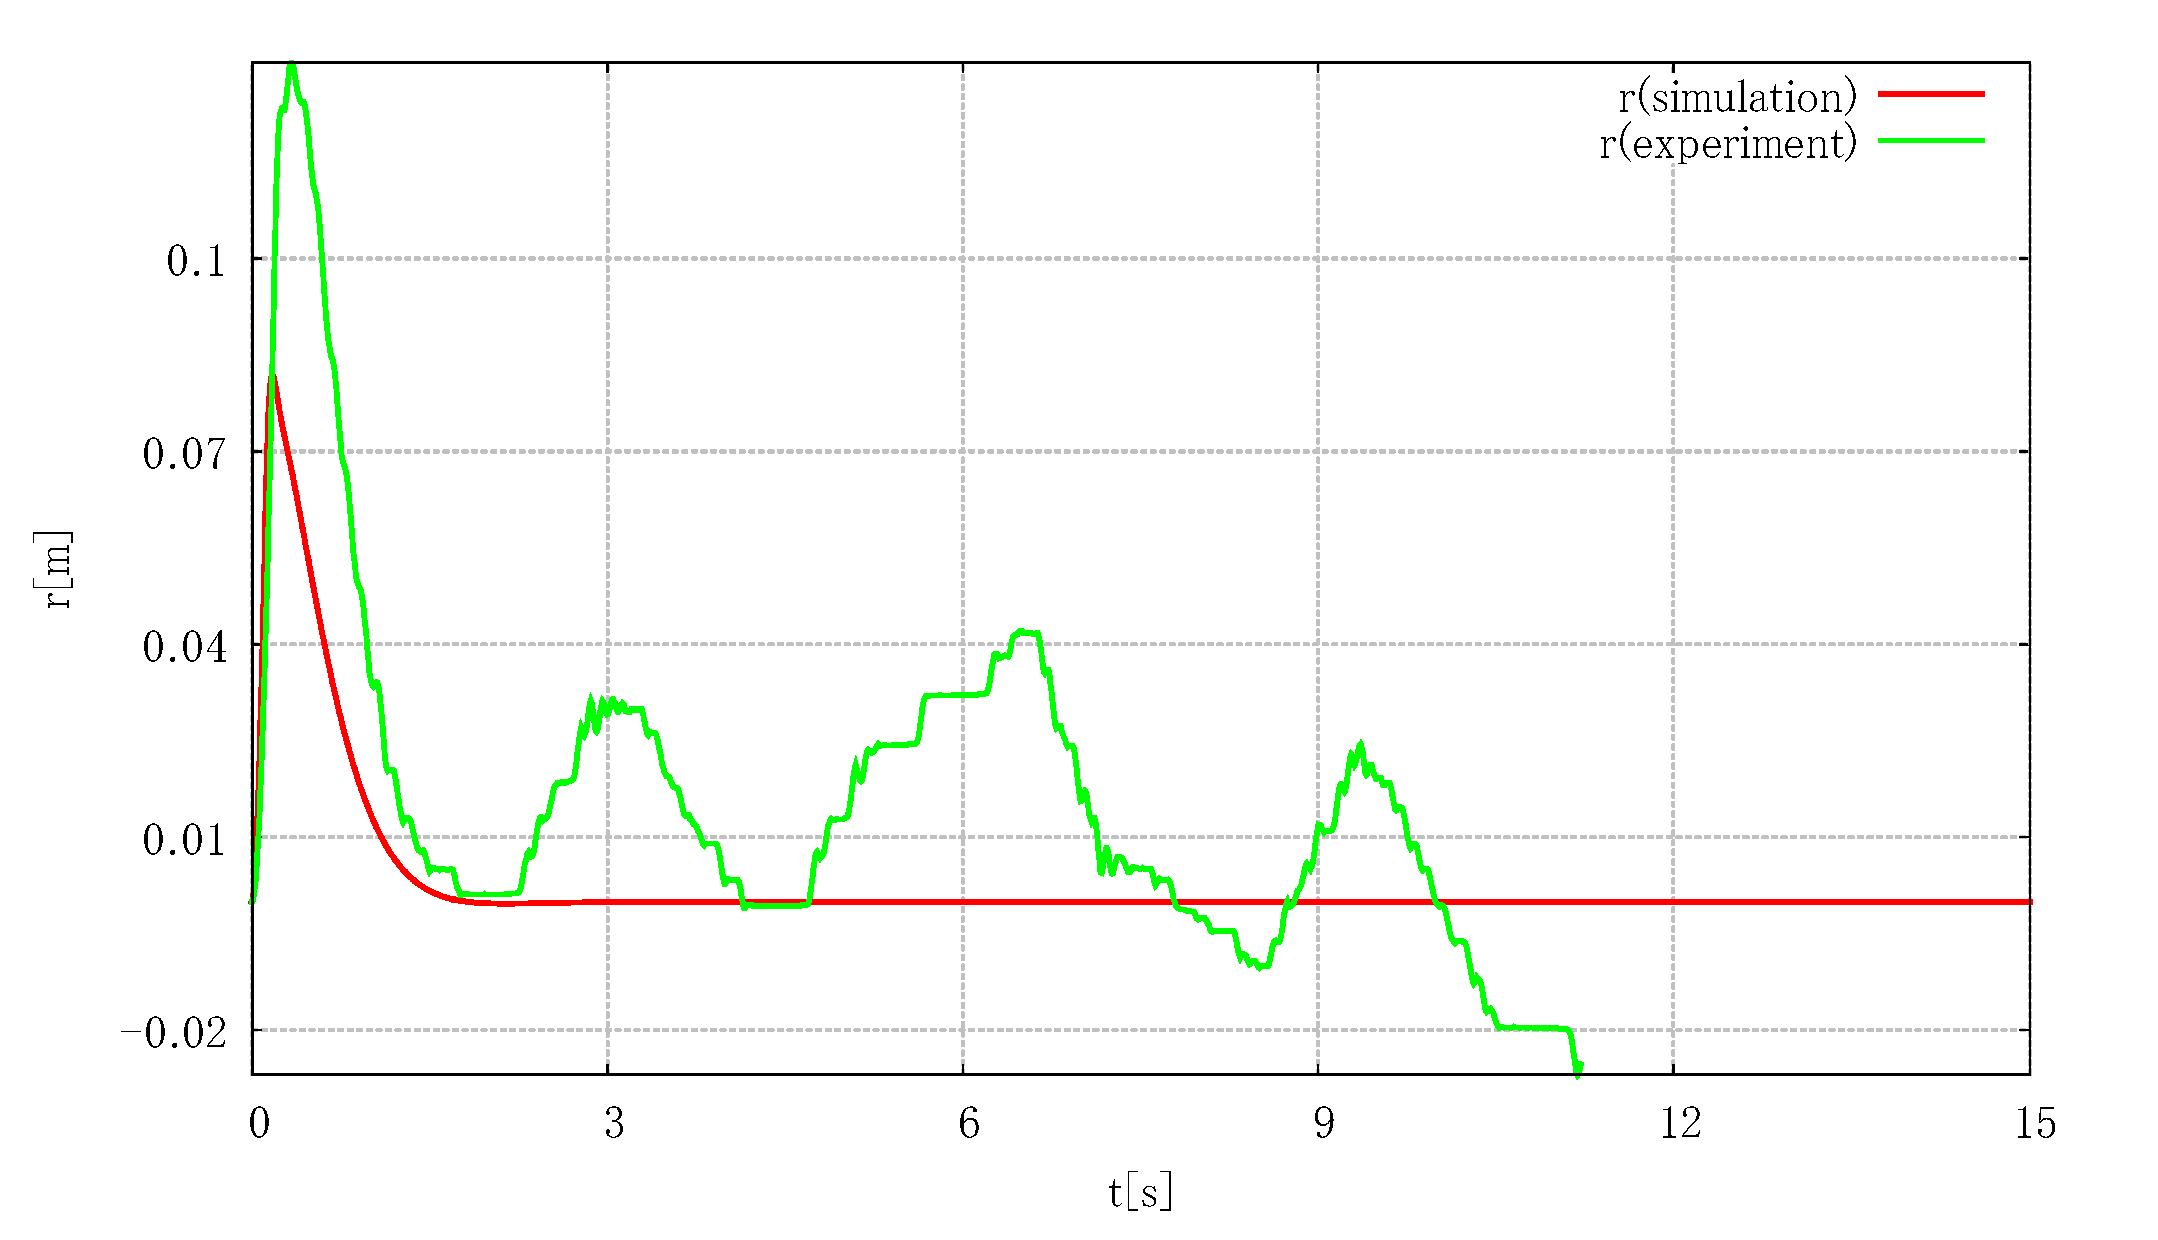
\includegraphics[width=0.8\linewidth]{gazo/experiment_control_R.eps}
		\caption{安定化制御実験結果(台車位置)}
		\label{image:experiment_control_R}
	\end{figure}
	\begin{figure}[H]
		\centering
		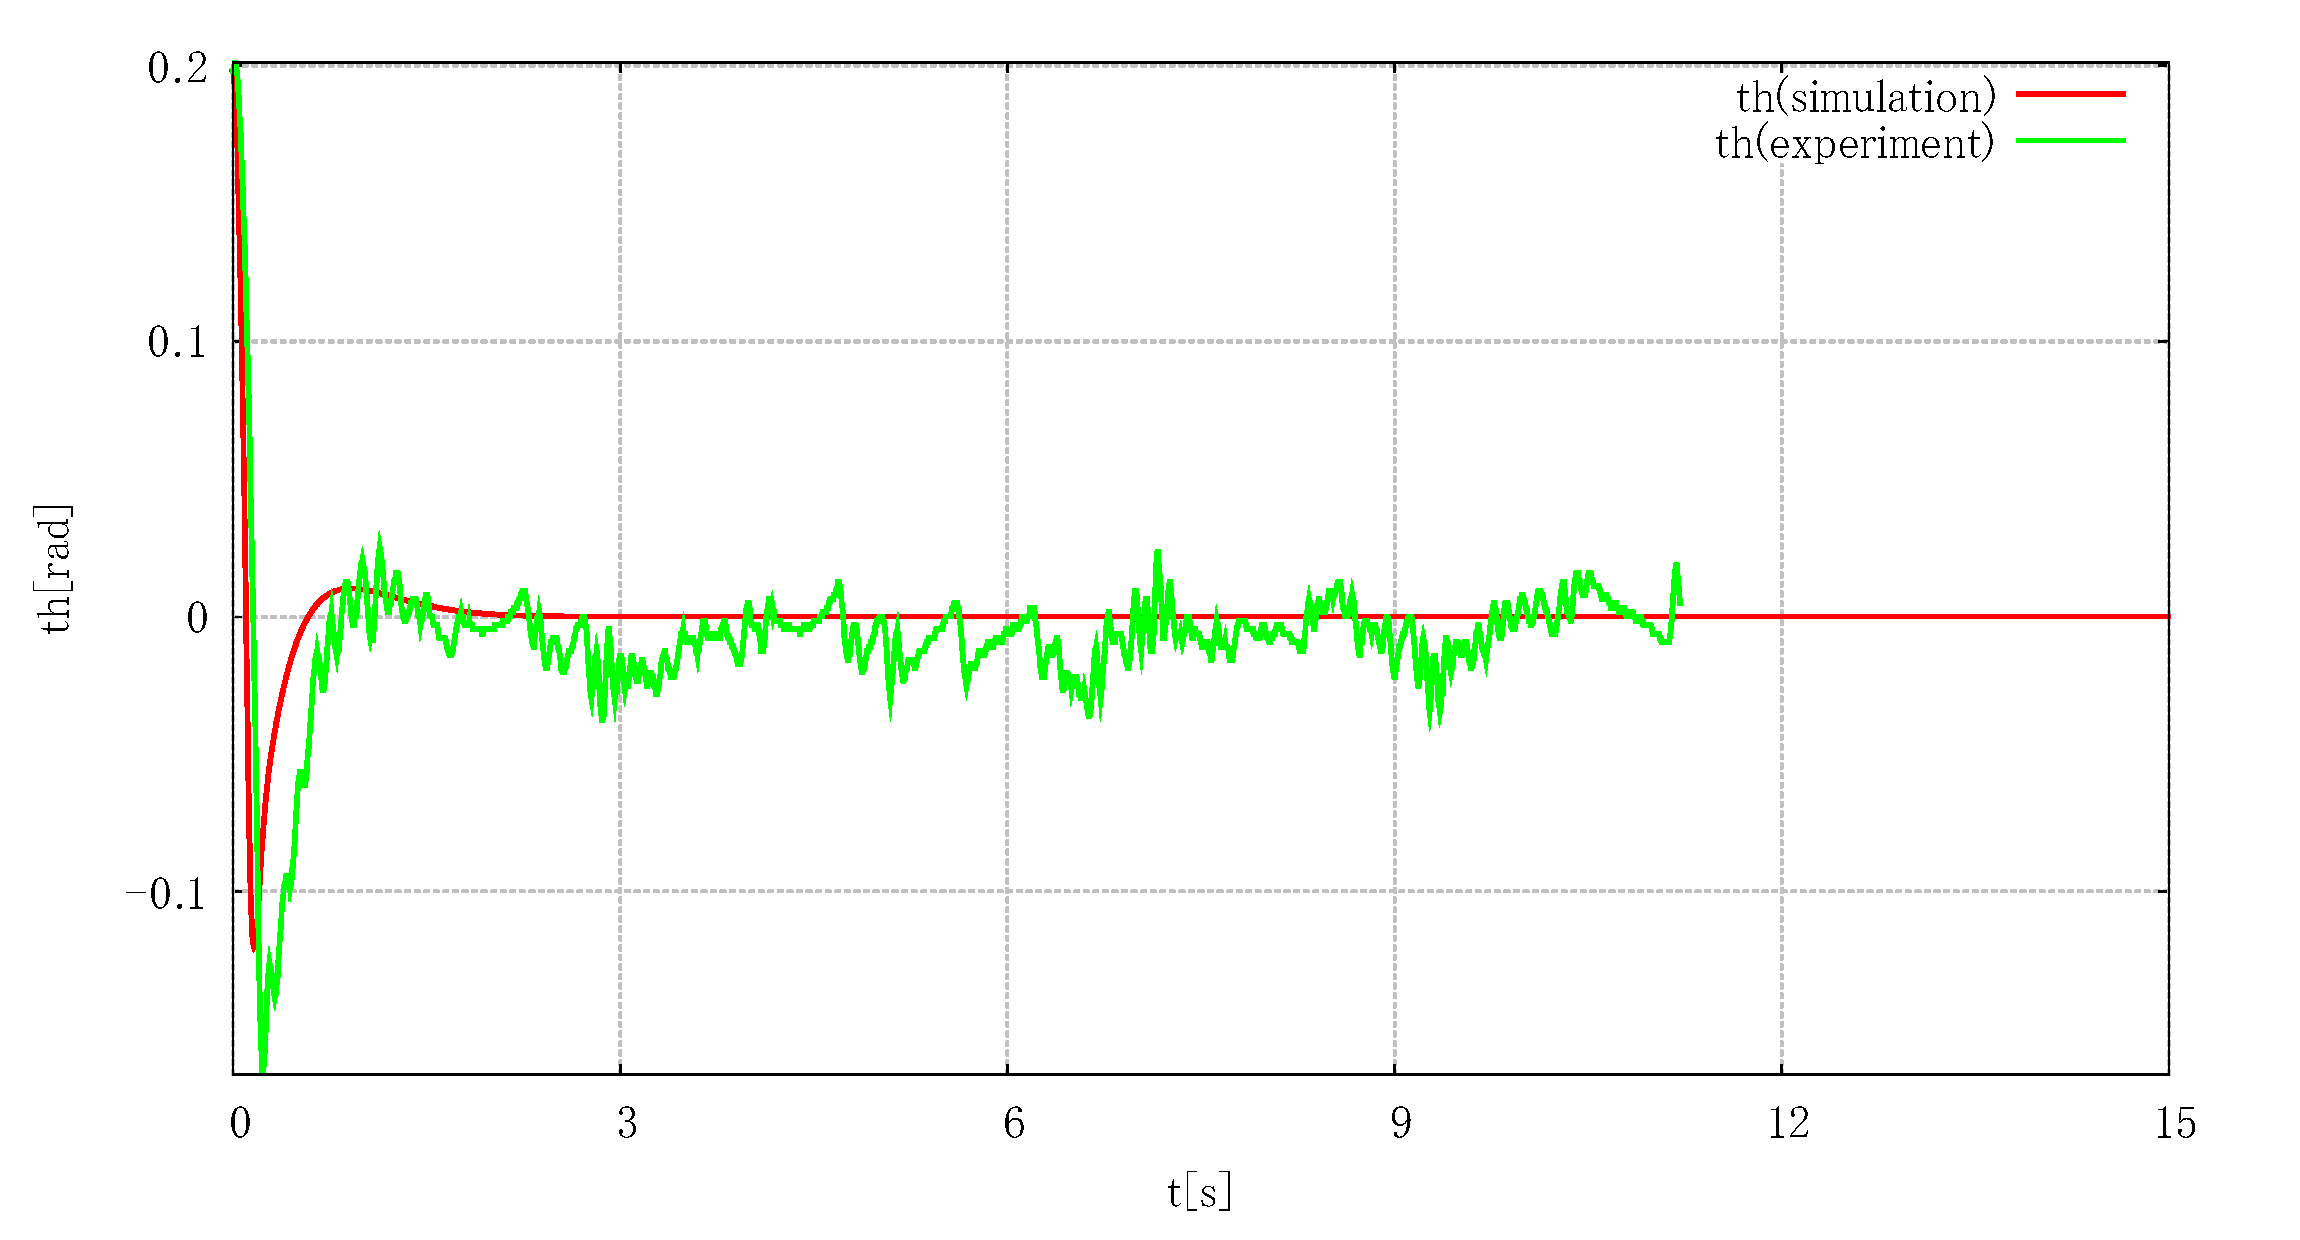
\includegraphics[width=0.8\linewidth]{gazo/experiment_control_TH.eps}
		\caption{安定化制御実験結果(振子角度)}
		\label{image:experiment_control_TH}
	\end{figure}
	図\ref{image:experiment_control_R}と図\ref{image:experiment_control_TH}
	より一番最初の山は実験のほうが大幅に大きくなっているのと、ノイズが乗っている点を除いてシミュレーションと実験結果は
	概ね一致しているといえる。これは、実験のほうではデータの計測を開始して振子から手を離したためその影響が出たといえる。
	この時の初期角度は$0.1979°$である。%radに直してほしいなぁ
	よって、初期角度がある程度ある中で実験を開始し、安定化制御を行うことができたため、
	実験目的の第一項目を達成できたといえる。
	
	
	
%-----------------------------------------------------------
\section{目標値の変更実験}
	台車に目標値を与えて、その目標値に台車が移動しても安定化制御可能か実験を行う。(実験項目の第二項目)
	なお、目標値は5秒ごとに0→0.1→0のように変更される。
	以下にその結果とシミュレーション結果との比較を行った図を示す。

%-----------------------------------------------------------
\section{振り上げ制御及び安定化実験}
	振子を真下に配置し、そこから台車の動きだけで振子を振り上げ、
	安定化制御が可能か実験を行う。(実験項目の第三項目)
	以下にその結果とシミュレーション結果との比較を行った図を示す。

%-----------------------------------------------------------